\chapter{Implementierung der Webanwendung}

%\section{Struktur der Webanwendung}
%\subsection{Benutzeroberfläche}
%Die Oberfläche der Anwendung beschränkt sich nur auf das Nötigste. Für die Eingabe von Daten werden lediglich Webkomponenten Inputs verwendet, welche durch die Nutzung von paper-inputs\footnote{https://www.webcomponents.org/element/PolymerElements/paper-input}, die der Materialdesignkonvention\footnote{Eine Anleitung, wie man Benutzeroberflächen und deren Komponenten gestalten sollte} folgen, passend gestaltet sind.

%\subsection{Server}
%Um einen Node.js Server mit dem Express Framework aufzusetzen und zu konfigurieren, wird, wie in Kap.~\ref{cha:scram-engine} erläutert, auf der Arbeit von Jordan Last aufgebaut und diese passend erweitert. 
%Die Client-Server-Kommunikation erfolgt mittels Ajax-Aufrufen durch die iron-ajax Komponente\footnote{https://www.webcomponents.org/element/PolymerElements/iron-ajax}.
%\subsection{Datenbank}
%Da es für Datenbankzugriffe, zum Zeitpunkt dieser Arbeit, keine vorhanden Webkomponenten gibt, sind eigenes welche für alle CRUD-Operationen entwickelt und umgesetzt worden.

%\subsection{Datenflow}
Die AnwenderInnen sollen zu beginn Datensätze anlegen können. Im konkreten Beispiel wurde das Datenmodell eines Users mit Username, E-Mail und Passwort herangezogen.
Nachdem die AnwenderInnen die Daten für einen User ausgefüllt haben, kann dieser angelegt werden. Nach rudimentären Validierungen werden die Daten an den Server übermittelt. Dieser speichert den User in der Datenbank ab. 
In der Listenansicht sieht der Anwender alle bereits angelegten User in einer Tabelle und per Klick auf dessen Namen wird zur Detailansicht weitergeleitet. Hier wird ein Formular mit den Userdaten ausgefüllt, welche verändert und aktualisiert werden können.   
Auf der Detailseite findet sich ebenso ein Lösch-Knopf, um einen bestehenden User zu entfernen.
\section{Umsetzung mit Dependencies Electron / Scram-Engine}
Um die Nutzung von Webkomponenten am Server zu ermöglichen, werden zwei konkrete Technologien benötigt, da Webkomponenten grundsätzlich nur im Browser funktionieren.
\subsection{Electron}
Electron ist ein Framework, um native Cross-Plattform-Applikationen mit Web-Technologien wie JavaScript, HTML und CSS zu erstellen. Es basiert auf dem Chromium\footnote{https://www.chromium.org/} Webbrowser und Node.js.
\subsection{Scram-Engine}
\label{cha:scram-engine}
Das Scram-Engine-Projekt, erarbeitet von Jordan Last, ermöglicht es, eine HTML-Datei einem vorkonfigurierten Electronstartscript mit minimalem Aufwand, zur Verfügung zu stellen. Es wird lediglich Electron von der Kommandozeile aufgerufen und eine Startdatei mitgegeben. Die Vorkonfiguration vereinfacht das Arbeiten mit Electron durch beispielsweise das Anbieten von Kommandozeilenargumenten, um das Electronfenster zu verstecken, und somit das bequeme Starten von serverseitigen Anwendungen aus der Kommandozeile heraus.
Electron ist notwendig, da es Chromium mit Node.js kombiniert. Die Scram-Engine nutzt Chromiums Fähigkeit, Webkomponenten in einen interaktiven DOM zu parsen, welcher manipuliert werden kann. Diese Webkomponenten können dadurch jeglichen Node.js Code nutzen und haben die Möglichkeit mit dem Betriebssystem zu interagieren, Datenbankaufrufe zu tätigen, prinzipiell alles, was Node.js möglich ist.
Ein reiner Node.js Server würde nicht ausreichen, da dieser HTML, Custom-Elemente oder Webkomponenten generell nicht parsen kann.
Durch die Kombination der beiden Technologien können Webkomponenten weitaus mehr leisten, als in einem Webbrowser.

Da universelle Webkomponenten auf Electron als deren Plattform angewiesen sind, muss das System, welches diese betreibt, relativ leistungsstark sein. Jordan Last arbeitet an einer Lösung, um die Electron-Abhängigkeit -- und dadurch die Chromium-Abhängigkeit -- loszuwerden. Jegliche Interessenten, die an dieser Optimierung mitwirken möchten, können ihn kontaktieren\footnote{https://github.com/lastmjs}.

\section{Implementierung der Komponenten}
Die Hauptteile, der für diese Arbeit entwickelten Prototypen, werden in Frontend und Backend eingeteilt. Wobei das Backend nochmal in Server und Datenbank unterteilt wird. 

\subsection{Frontend}
Im Frontend wurde hauptsächlich auf bereits vorhanden Webkomponenten aufgebaut. Es wurden Standard HTML-Elemente durch paper-input Elemente\footnote{https://www.webcomponents.org/collection/PolymerElements/paper-input-elements} ersetzt, um ein abgestimmtes Gesamtbild zu erzeugen, ohne sich auf das Design konzentrieren zu müssen. So wurde bei dem Anlegen eines neuen Nutzers, wie in Abb. \ref{fig:user_create} ersichtlich, auf <paper-input> Elemente mit einem <iron-icon> Element gesetzt. Das Aktualisieren eines Nutzers ist das selbe Formular, lediglich mit anderen <paper-button> Komponenten. Die Auflistung, aller bereits erstellten Nutzer, wurde durch ein <paper-datatable-api> Element erstellt. Jegliche Kommunikation zwischen Frontend und Backend wurde über eine REST-API gehandhabt. Die Anfragen wurde durch die <iron-ajax> Komponente vollzogen, welche eine Webkomponente für einfache ajax-Anfragen ist.
\begin{figure}
	\centering
	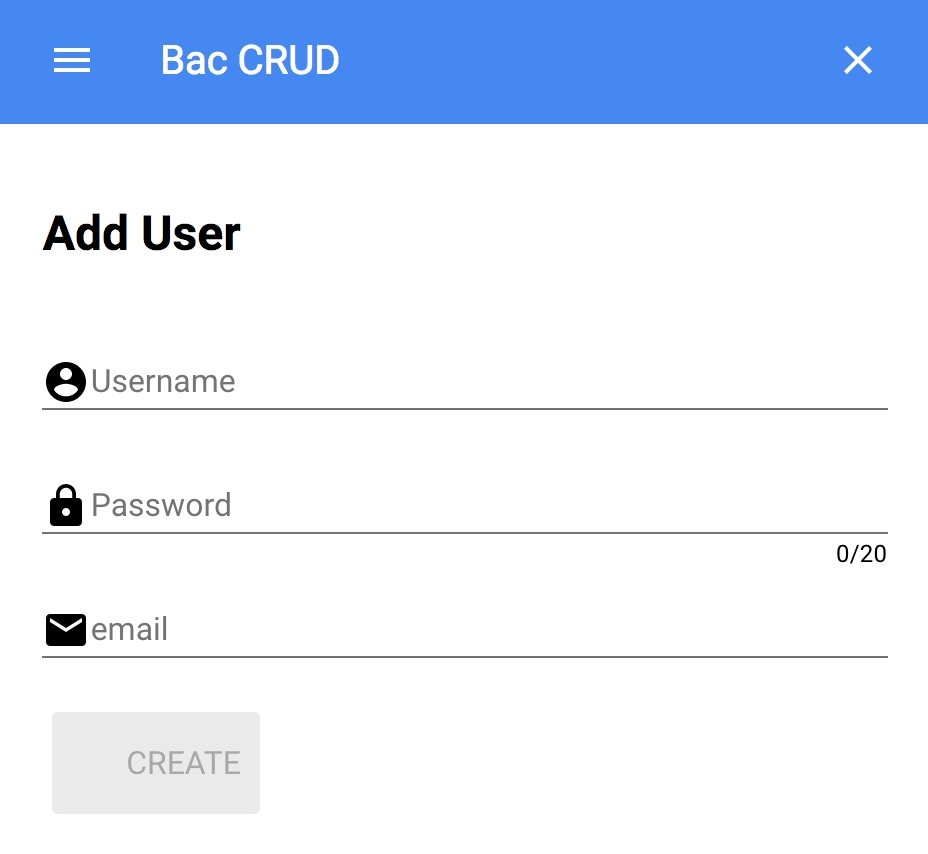
\includegraphics[width=0.5\linewidth]{images/user_create.jpeg}
	\caption{User erstellen}
	\label{fig:user_create}
\end{figure}

\begin{figure}
	\centering
	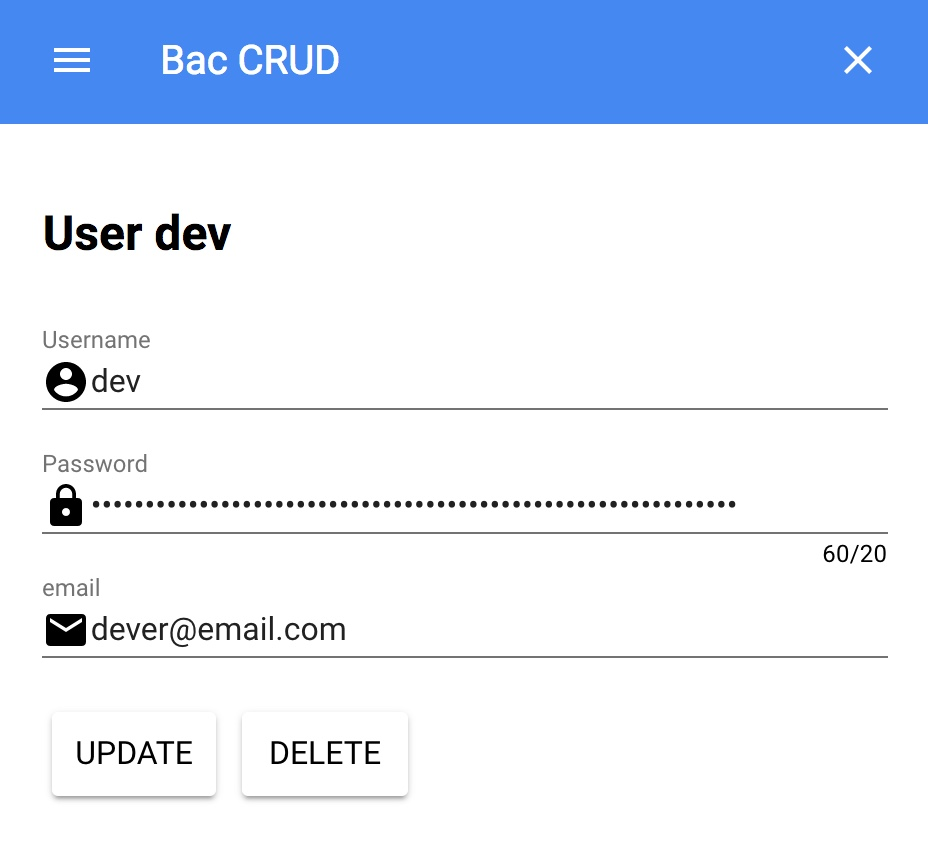
\includegraphics[width=0.5\linewidth]{images/user_update.jpeg}
	\caption{User bearbeiten}
	\label{fig:user_update}
\end{figure}

\begin{figure}
	\centering
	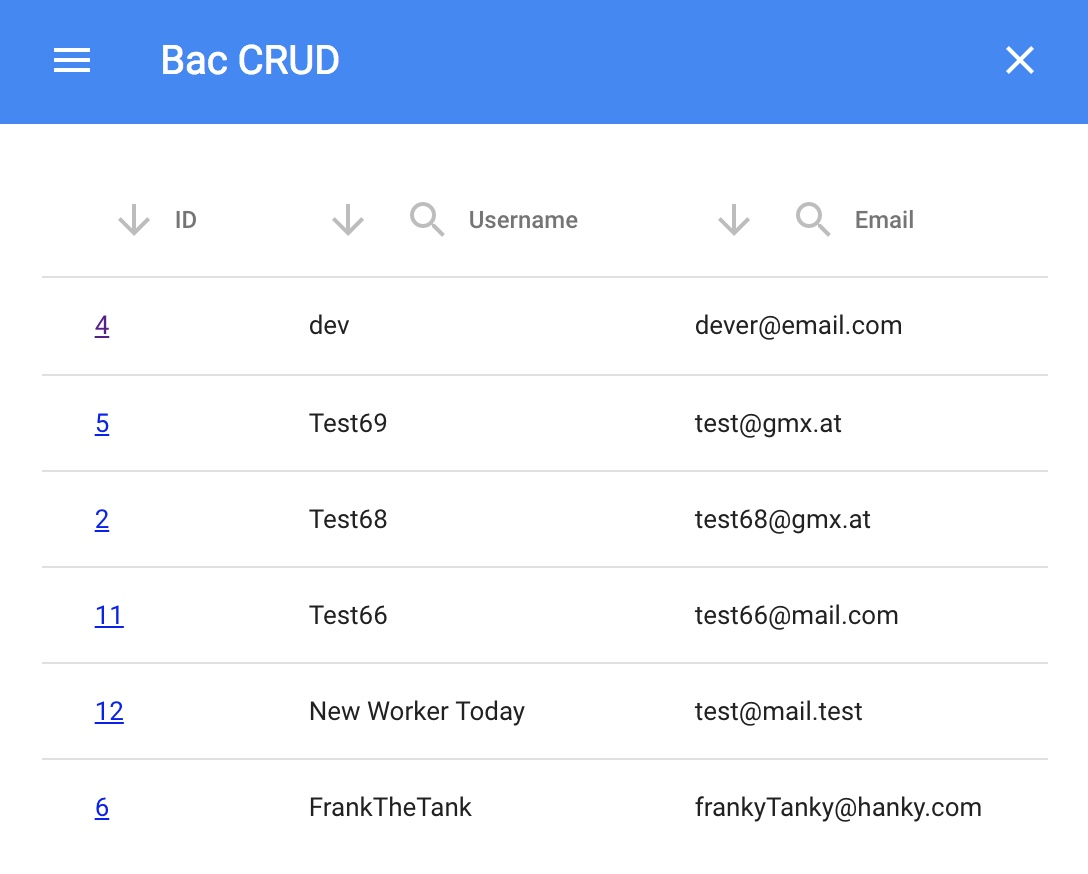
\includegraphics[width=0.5\linewidth]{images/user_list.jpeg}
	\caption{User Liste}
	\label{fig:user_list}
\end{figure}

\subsection{Server}
Anstatt, dass man REST-Routen in Javascript imperativ definiert, können diese deklarativ in HTML zusammen gebaut werden. Es wird so eine visuelle Hierarchie der vorhanden Routen erstellt. Durch die Visualisierung mit HTML behält man nicht nur den Überblick\footnote{hier durch die Formatierung eventuell nicht ersichtlich}, es ist auch einfacher zu verstehen, als das Äquivalent in Javascript.
Wie im Programm \ref{prog:server-config} ersichtlich, sind alle Endpunkte und Middlewares, welche die Express-Anwendung manipulieren, unter einem <express-app> Element verschachtelt. In der Reihenfolge, wie die Middlewares definiert werden, werden diese auch in die Anwendung eingepflegt. In einem <express-router> Element können ebenfalls <express-route> Elemente und Middlewares verschachtelt, und so komplexe Routen-System erstellt werden.
Hier wird beispielsweise in Zeile \ref{line:indexHandler} der \textit{indexHandler} als \textit{Callback} an ein <express-middleware> Element übergeben, welches eine Methode(\textit{get}) und einen Pfad(\textit{/})  besitzt. Diese Middleware befindet sich unter dem <express-router> mit der Basisroute als Pfad. Das bedeutet, dass dieser Router für seinen Pfad unter sich Routen haben kann, die ebenso einen Pfad besitzen. Da der \textit{indexHandler} auf die Basisroute angewendet werden soll, wird dieser Middleware ebenfalls die Basisroute als Pfad mitgegeben.

Die gezeigten Routen im Code  \ref{prog:server-config} sind rein zur Definition, welche URL, welche Seite rendern soll. Für REST-Anfragen, die Daten aus der Datenbank manipulieren, wurde eine eigene Komponente <db-router> erstellt, welche alle relevanten Datenbankanfragen verarbeitet\footnote{Die Funktionen der anderen verwendeten Middlewares können im Programmcode nachgeforscht werden}.

\begin{program}
\caption{Server Konfiguration mit Komponenten}
\label{prog:server-config}
\begin{HtmlCode}
<template>
	<express-app port="[[port]]">
		<express-config callback="[[staticMW]]"></express-config>
		<express-middleware callback="[[bodyParserMW]]"></express-middleware>
		<express-middleware callback="[[bodyParserUrlMW]]"></express-middleware>
		<express-middleware callback="[[cookieParserMW]]"></express-middleware>
		<express-middleware callback="[[sessionMW]]"></express-middleware>
		<express-config callback="[[cookieMW]]"></express-config>
		<express-router path="/">
				<express-middleware method="get" path="/" callback="[[indexHandler]]"></express-middleware>\label{line:indexHandler}
				<express-middleware method="get" path="/login" callback="[[loginHandler]]"></express-middleware>
				<express-middleware method="get" path="/logout" callback="[[logoutHandler]]"></express-middleware>
		</express-router>
		<express-router path="/user">
				<express-middleware method="get" path="/list" callback="[[userListHandler]]"></express-middleware>
				<express-middleware method="get" path="/new" callback="[[userCreateHandler]]"></express-middleware>
				<express-middleware method="get" path="/:id" callback="[[userDetailsHandler]]"></express-middleware>
		</express-router>
		
		<db-router></db-router>
		
		<express-middleware callback="[[undefinedPageMW]]"></express-middleware>
		
		<express-config callback="[[handleEndpoint]]"></express-config>
	</express-app>
</template>
\end{HtmlCode}
\end{program}

\subsection{Datenverwaltung}
Der im Programm \ref{prog:server-config} ersichtliche <db-router> verarbeitet jegliche REST-Anfragen und triggert <db-query> Komponenten, um Daten der Datenbank zu manipulieren. Diesem Element wird durch Kindelemente gesagt, was es für Abfragen tätigen soll. Besitzt das <db-query> Element lediglich ein <db-find> Element, wird davon ausgegangen, dass ein Datensatz von der Datenbank gesucht und zurückgegeben werden soll. Besitzt es aber zusätzlich zu dem <db-find> beispielsweise ein <db-delete>, so wird das <db-query> Element nicht den gefunden Datensatz zurückgeben, sondern löschen. 
 
\begin{program}
\caption{Datenverwaltung mit Komponenten}
\label{prog:datenverwaltung}
\begin{HtmlCode}
<db-query id="queryListUsers" db-model="[[userModel]]">
		<db-find></db-find>
		<db-sort sort2-query="{{_sort}}" sort-query="[[_sort]]" sort-property="username"
		sort-direction="asc"></db-sort>
</db-query>
	
<db-query id="queryUserDetails" db-model="[[userModel]]">
		<db-find find-query="[[findUserQuery]]"></db-find>
</db-query>
	
<db-query id="querySaveUser" db-model="[[userModel]]">
		<db-save save="[[newUser]]"></db-save>
</db-query>
	
<db-query id="queryUpdateUser" db-model="[[userModel]]">
		<db-find find-query="[[findUserQuery]]"></db-find>
		<db-save save="[[updateUser]]"></db-save>
</db-query>
	
<db-query id="queryDeleteUser" db-model="[[userModel]]">
		<db-find find-query="[[findUserQuery]]"></db-find>
		<db-delete></db-delete>
</db-query>
\end{HtmlCode}
\end{program}

\subsubsection{DB Query Komponente}
Um die interne Arbeitsweise zu verdeutlichen, wird die im Zuge dieser Arbeit entwickelte Webkomponente erläutert. Der exakte Programmcode kann auf GitHub nachgelesen werden\footnote{https://github.com/drdreo/webcomponent-cms/blob/master/server/components/db-query.html}. 
Als Parameter benötigt das <db-query> Element eine eindeutige ID, welcher zum Auslösen der Abfrage benötigt wird, und das zugehörige  Datenbankmodell, da dieses Element für mongoDB mit mongoose entworfen wurde.
Die Komponente ist so konzipiert, dass diese zu Beginn durch alle Kindelemente traversiert, die unterschiedlichen Typen überprüft und abhängig von den vorhanden DB-Element-Typen die Element-Parameter zur eigentlichen \textit{Query} zusammenfügt. Mit einer Funktion, welche als Parameter eine Callback-Funktion mitbekommt, kann die  \textit{Query} ausgelöst und auf das Resultat reagiert werden.

